\documentclass[final,11pt,oneside,UTF8]{report}
\usepackage{ctex}
\usepackage{float}
\usepackage{geometry}
\usepackage{graphicx}
\usepackage{mhchem}
\usepackage{amsmath,amsfonts,amssymb}
\title{猪心解剖实验报告}
\author{Andy Shen}
\date{11th.Dec.2021}
\begin{document}
\maketitle
\section{实验准备}
\paragraph{
    为了进行这个实验,我准备了$1mol\cdot L^{-1}$的柠檬酸钠溶液进行抗凝(防止血块干扰观察),
    一个猪心,一把解剖剪刀,一把解剖刀,一把镊子,如下图所示
}
\begin{center}
    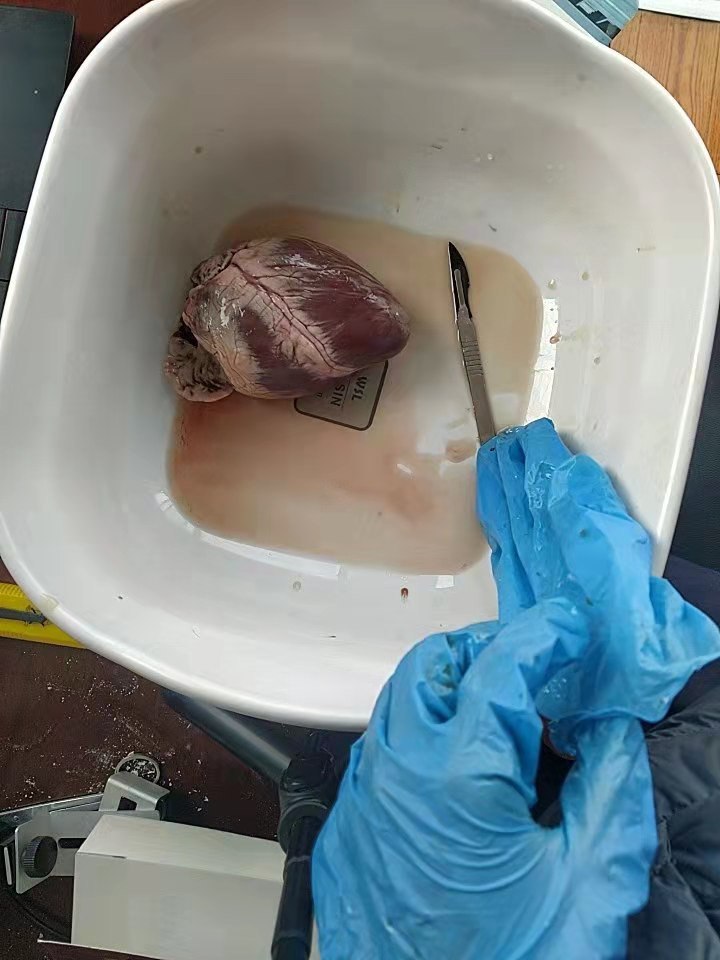
\includegraphics[scale=0.12,angle=0]{photos/start.jpg}
\end{center}
\paragraph{
    先直接观察一下主动脉和肺动脉以及动脉瓣,如图所示,被镊子夹出的就是主动脉动脉瓣,所对应的
    就是主动脉:
}
\begin{center}
    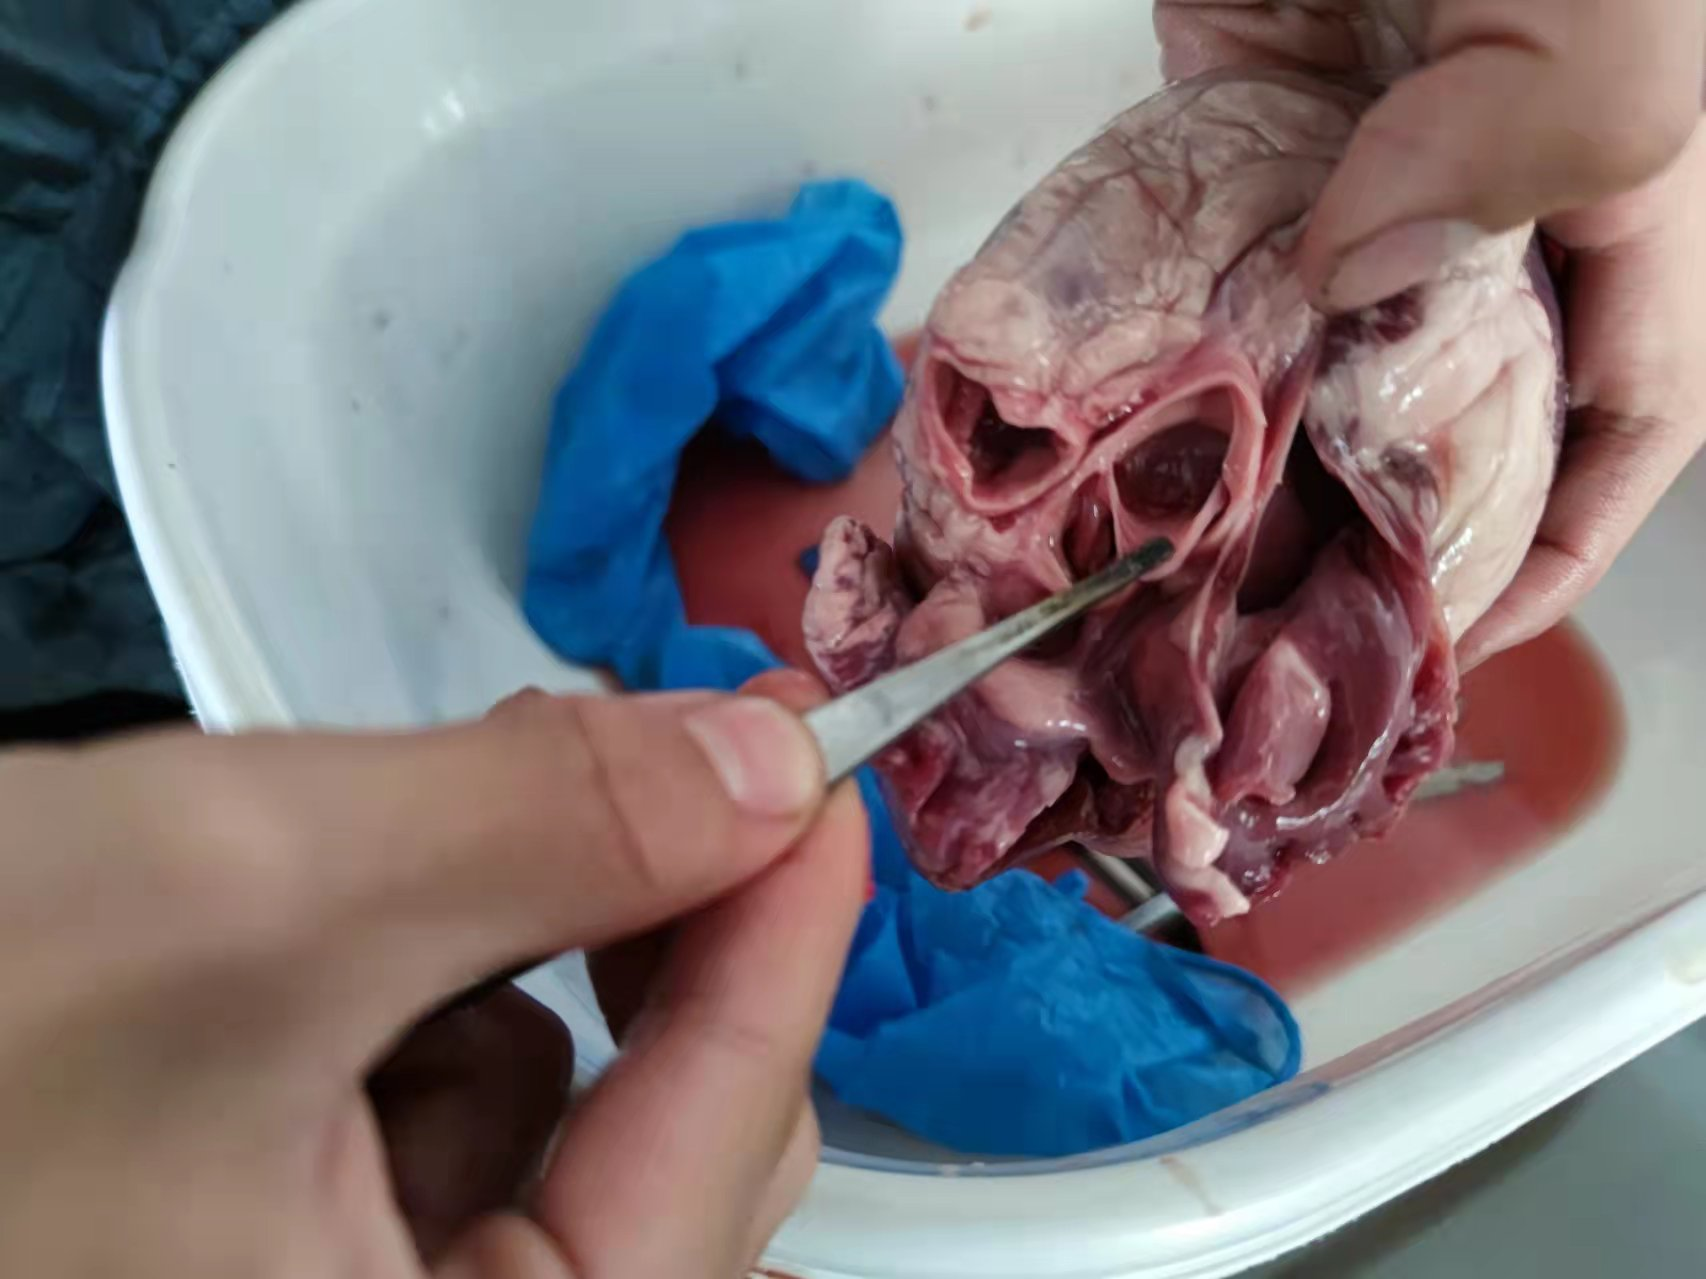
\includegraphics[scale=0.1,angle=0]{photos/main.jpg}
\end{center}
\paragraph{
    同理,这个就是肺动脉:
}
\begin{center}
    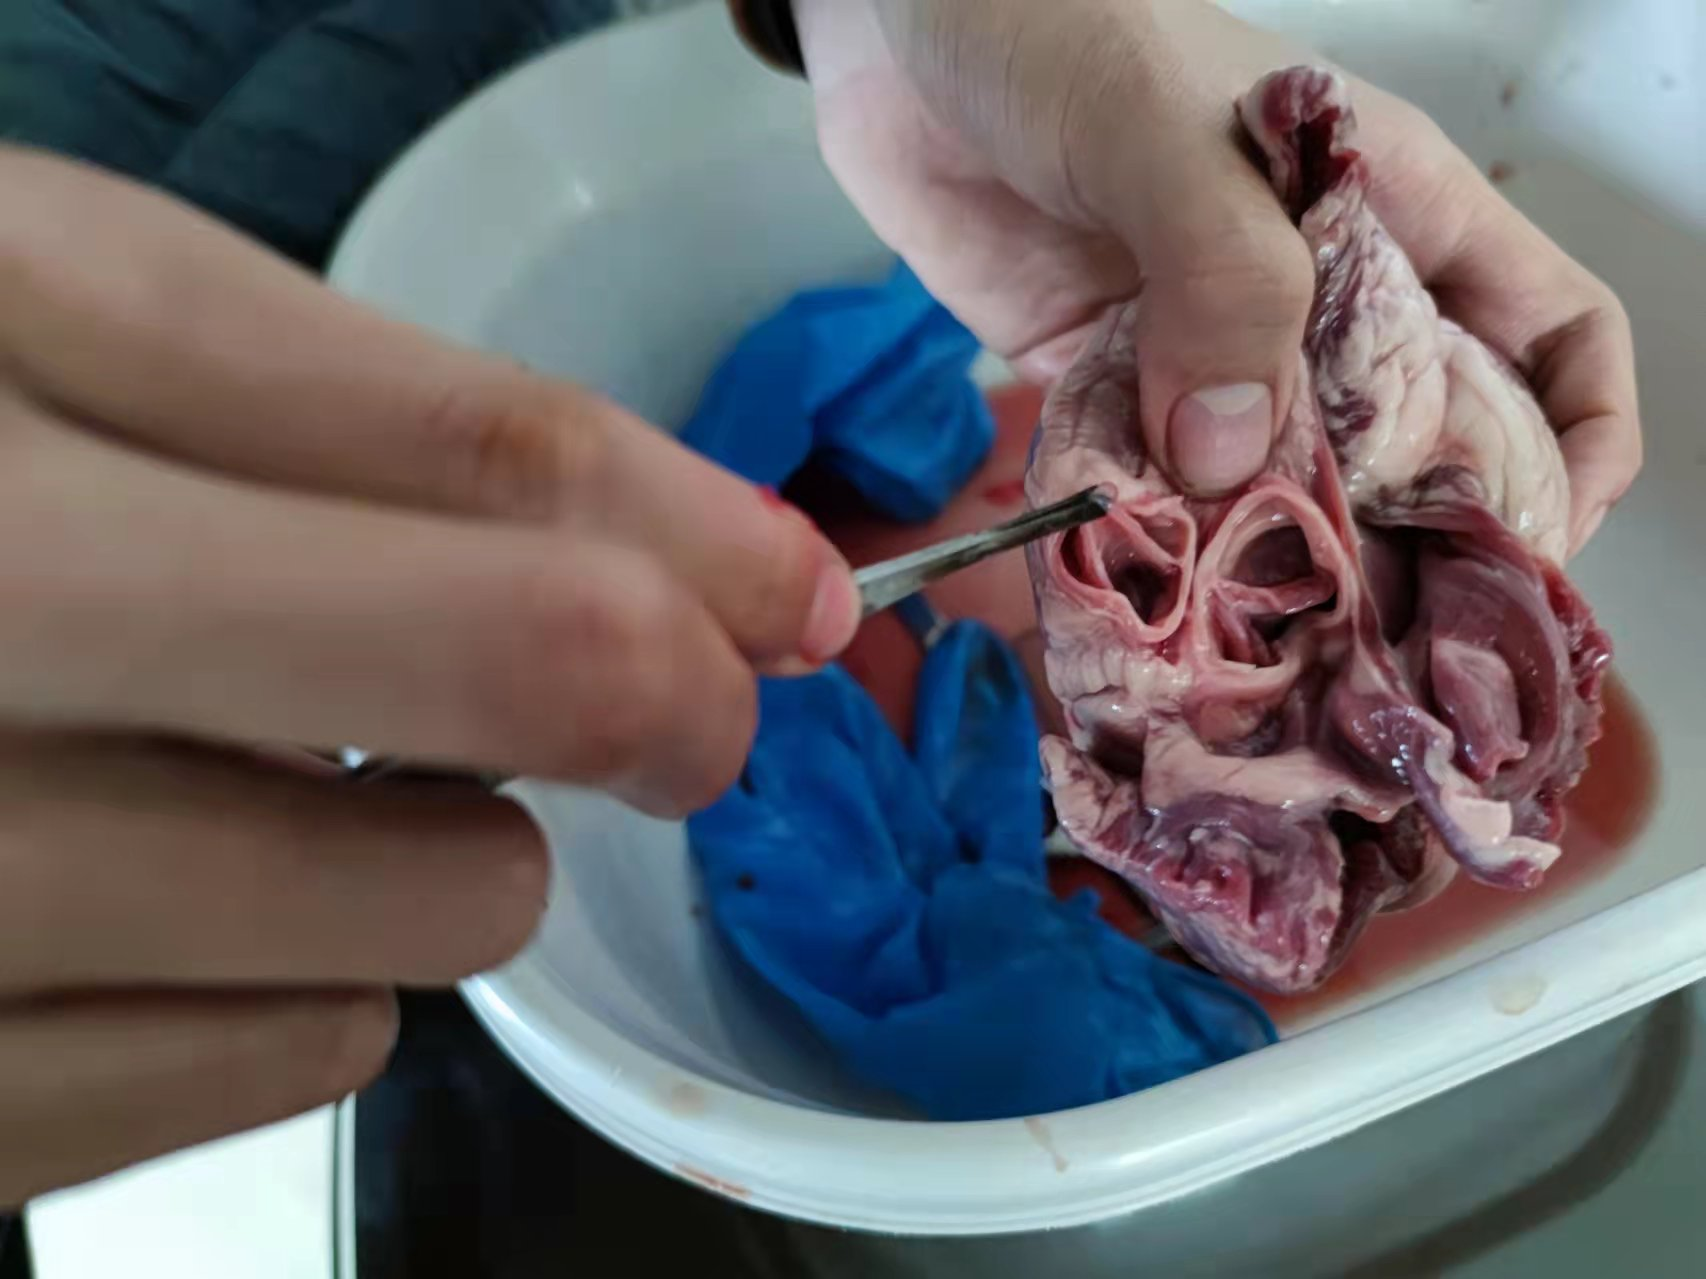
\includegraphics[scale=0.1,angle=0]{photos/lung.jpg}
\end{center}
\section{开始解剖}
\paragraph{
    开始解剖,先在血管中倒入柠檬酸钠溶液静置以溶血。然后使用解剖刀切开右心。然后使用大拇指穿过
    发现能够直接从右心室插到肺动脉,如图所示:
}
\begin{center}
    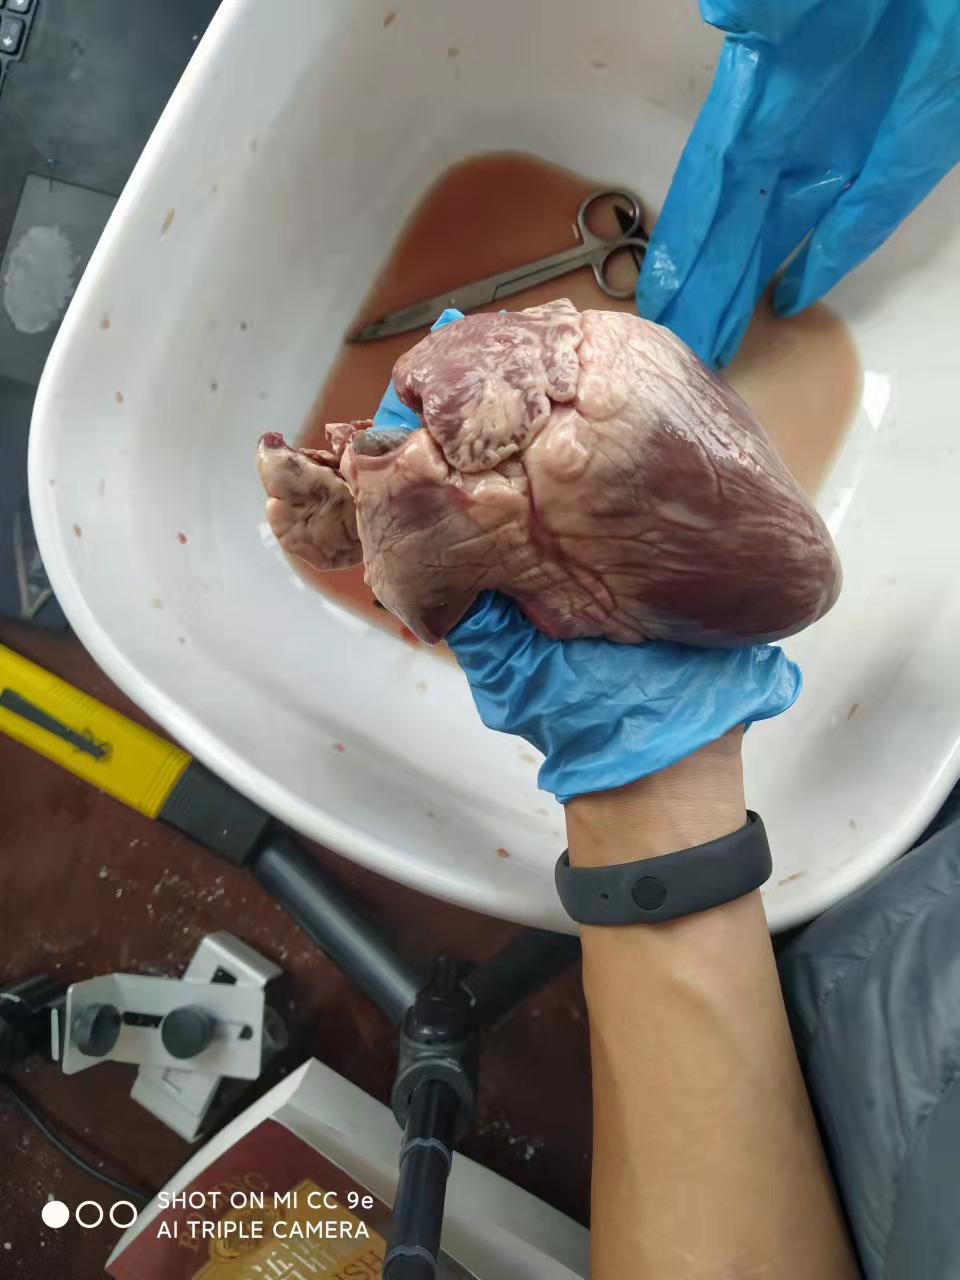
\includegraphics[scale=0.1,angle=0]{photos/stickR.jpg}
\end{center}
\paragraph{
    类似的,切开左心室,将手指插入,同样能够插到主动脉,如图所示。
}
\begin{center}
    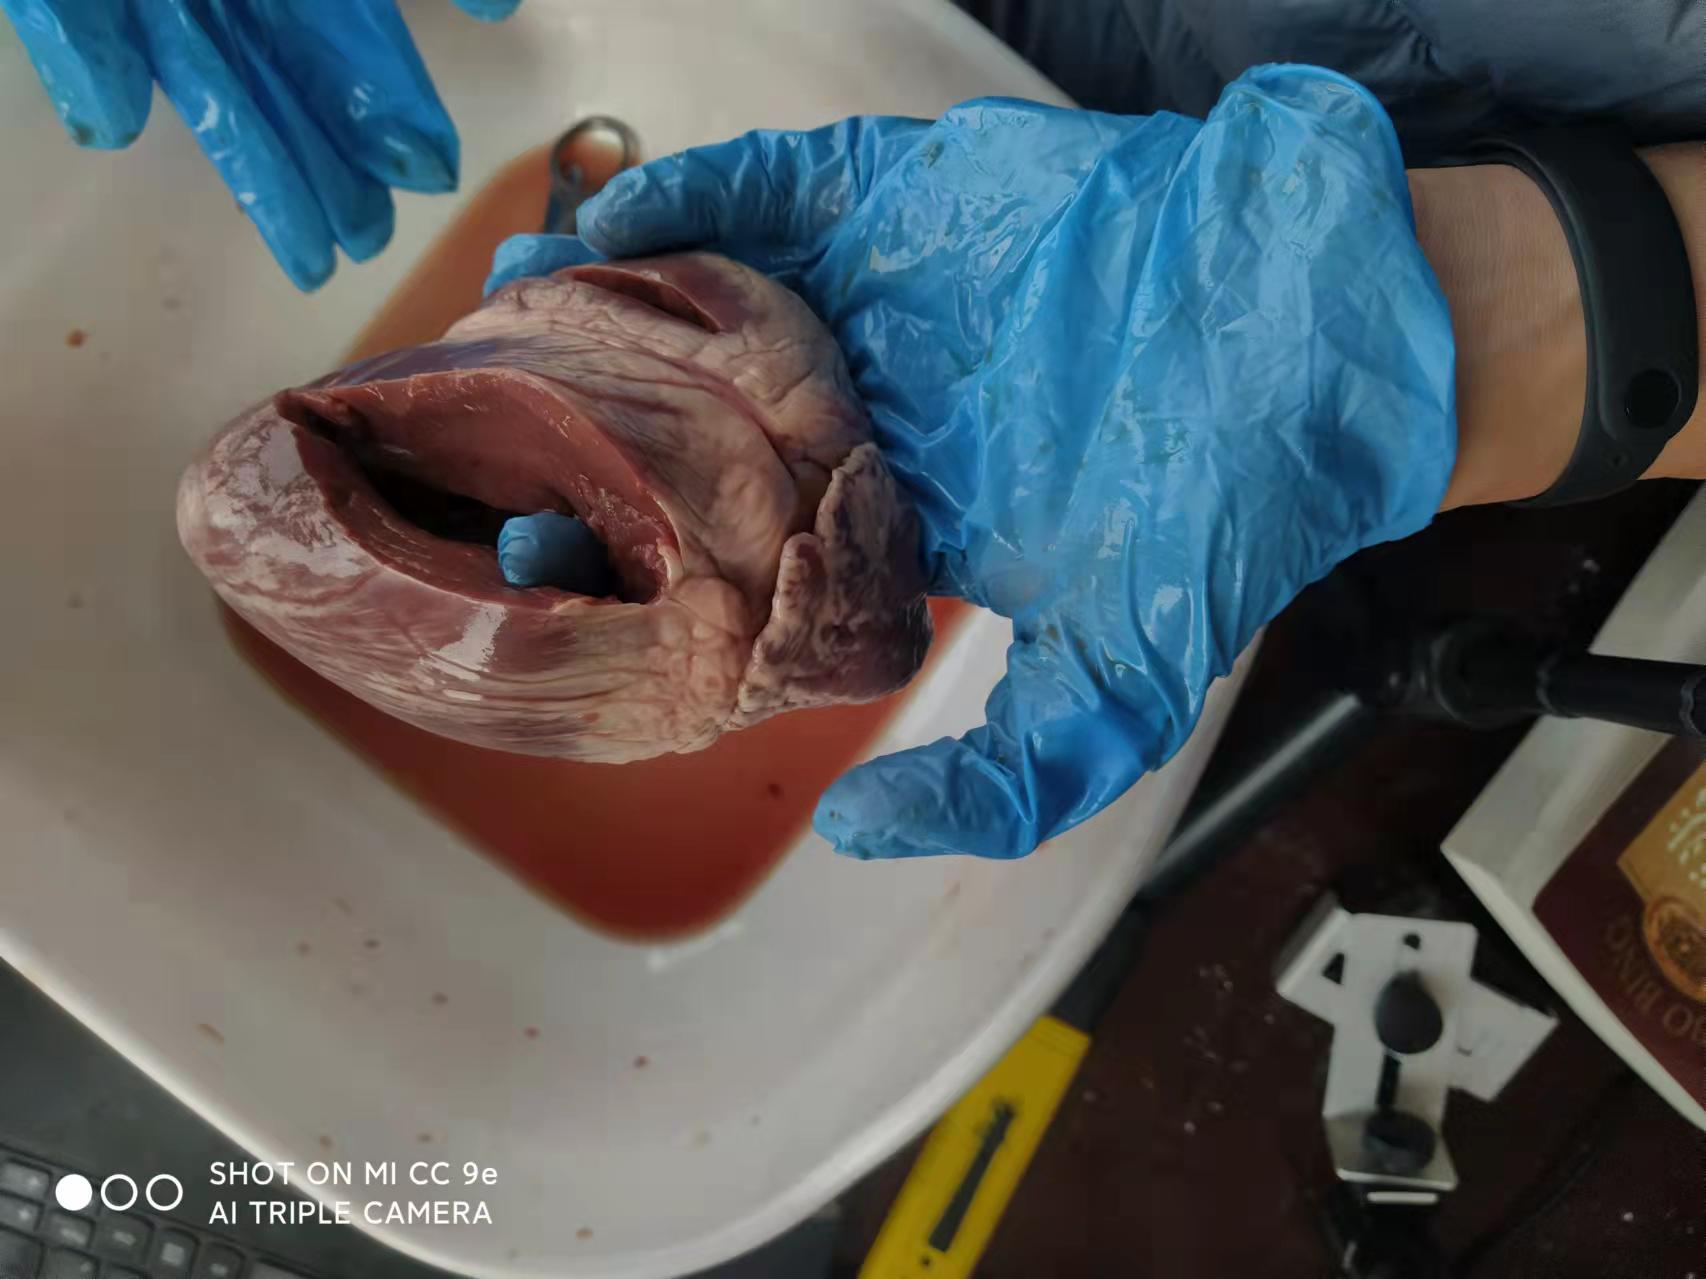
\includegraphics[scale=0.1,angle=0]{photos/stickL.jpg}
\end{center}
\paragraph{
    此时我在好奇,房室瓣在何处。通过查阅资料,看到下面两幅图,大概知道了房室瓣的位置
}
\begin{center}
    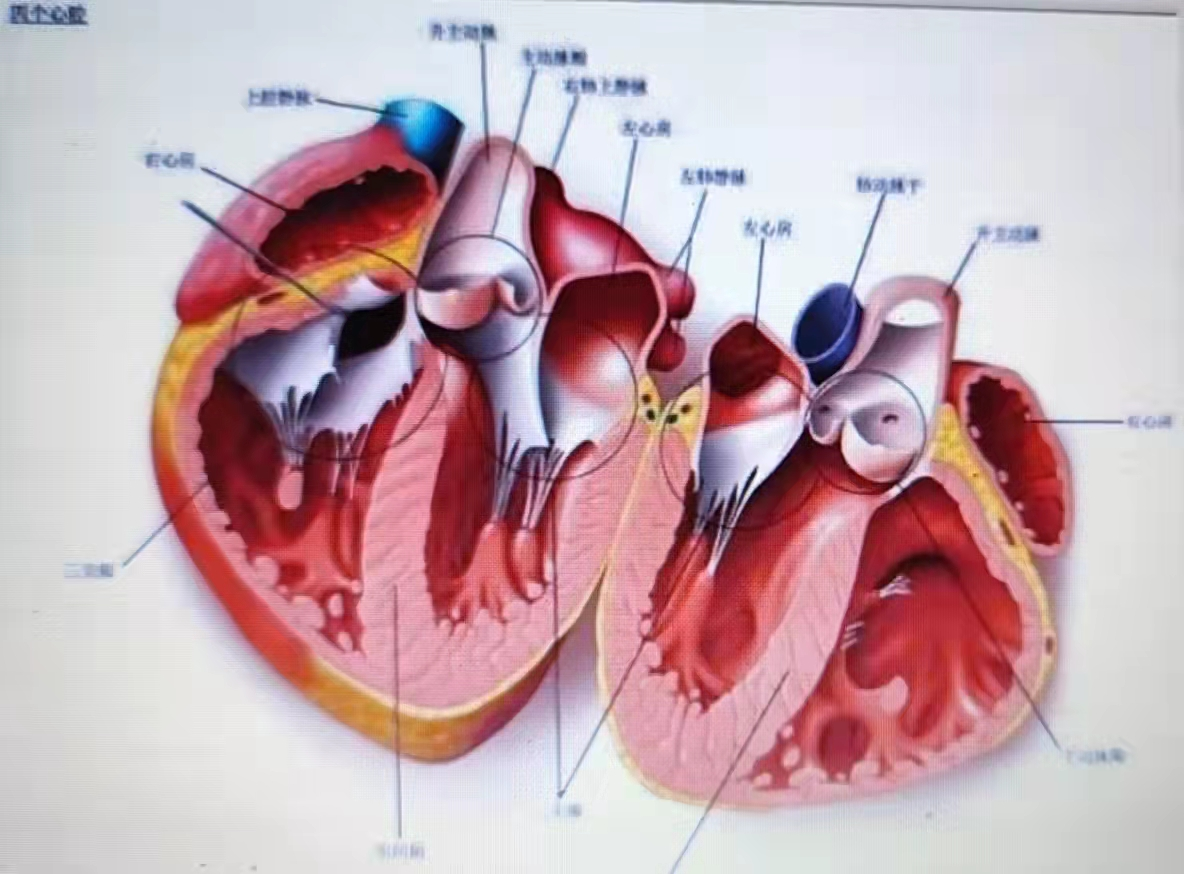
\includegraphics[scale=0.1,angle=0]{photos/example1.jpg}
\end{center}
\begin{center}
    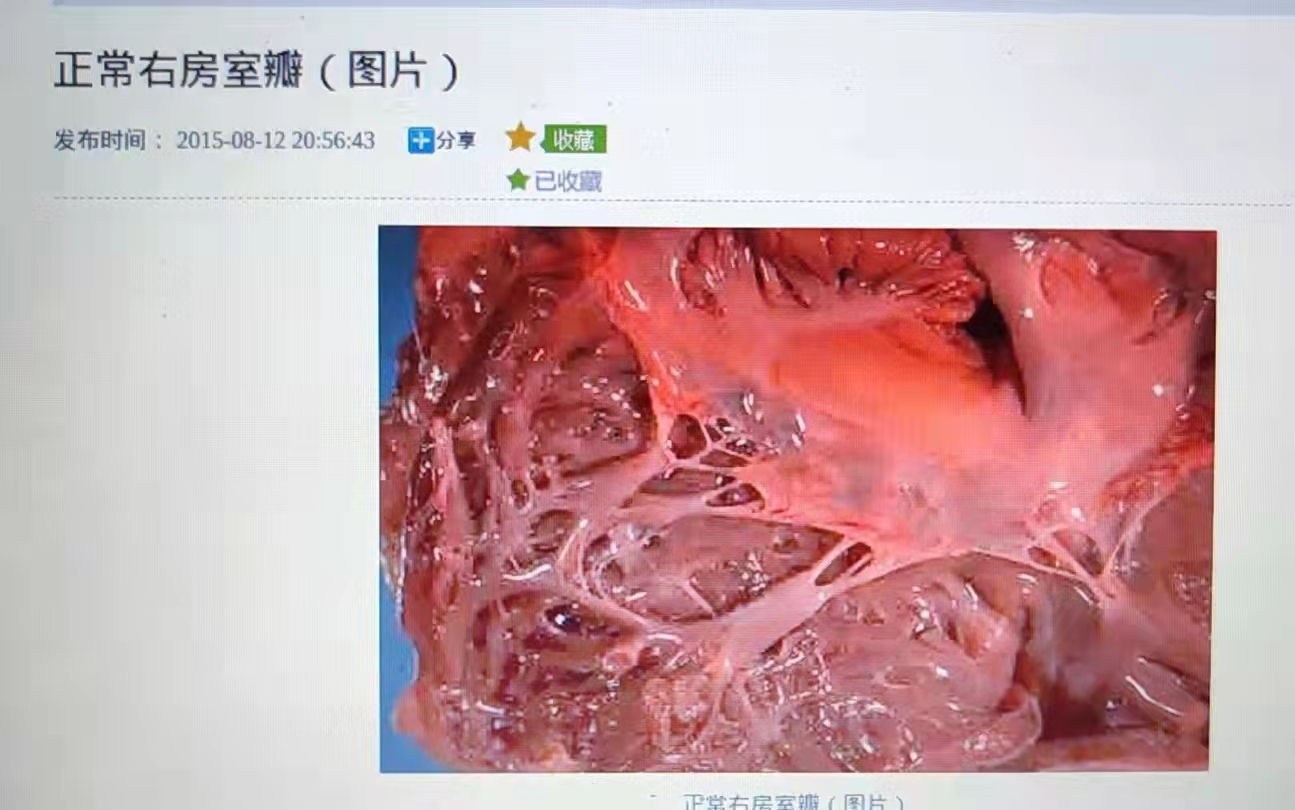
\includegraphics[scale=0.1,angle=0]{photos/example2.jpg}
\end{center}
\paragraph{
    在有理论的情况下,继续剪开两个心室,并用力扒开,如下列图所示,用镊子夹出的均为房室瓣
}
\begin{center}
    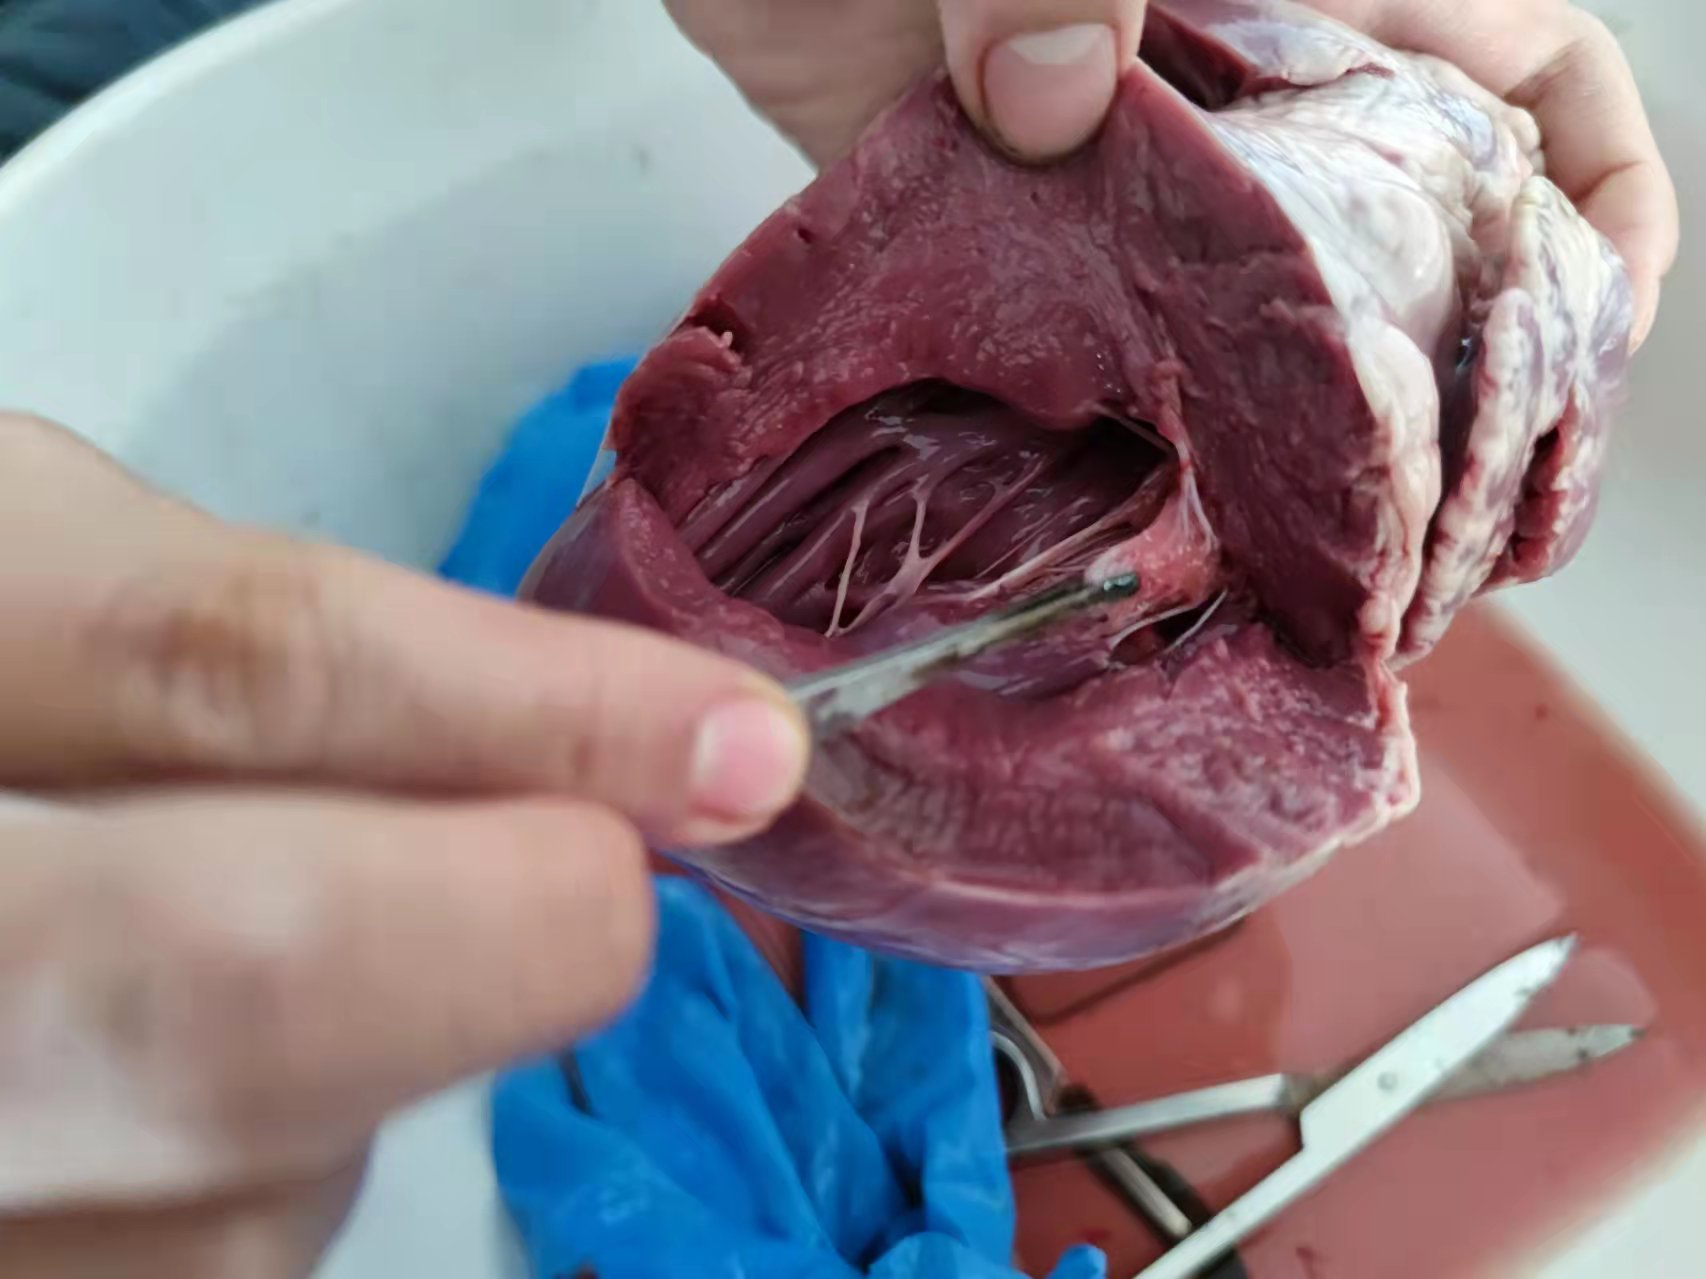
\includegraphics[scale=0.1,angle=0]{photos/Rm.jpg}
\end{center}
\begin{center}
    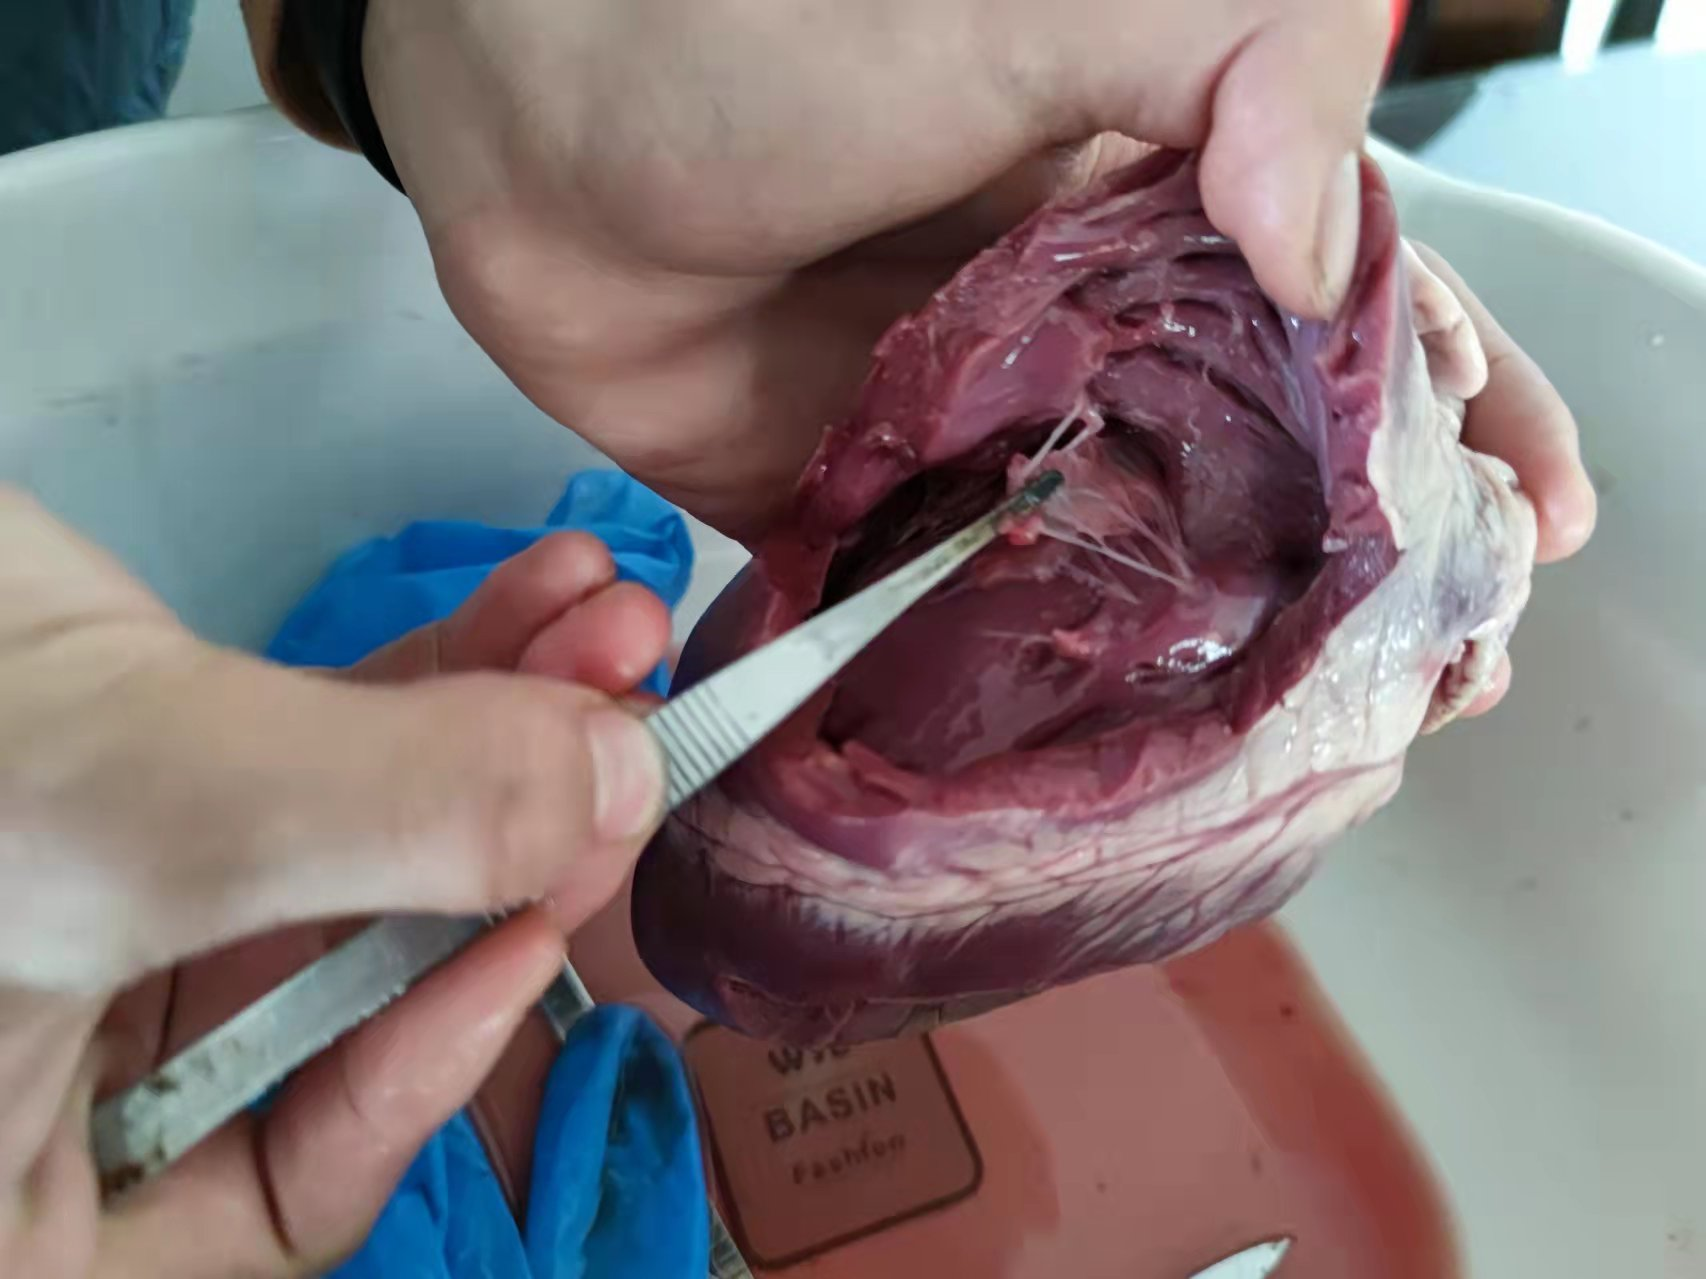
\includegraphics[scale=0.1,angle=0]{photos/Lm.jpg}
\end{center}
\paragraph{
    由于肺静脉没有保留完整,故没法进行该实验,从肺静脉注水应该能够溢出,同样的,从肺动脉注水
    也会溢出,故静脉瓣动脉瓣房室瓣的作用均是防止血液倒流。
}
\end{document}